\documentclass[UTF-8]{ctexart}
\usepackage{geometry}
\usepackage{graphicx}
\usepackage[namelimits]{amsmath} %数学公式
\usepackage{amssymb}             %数学公式             %数学字体
\usepackage{mathrsfs} 
\usepackage{txfonts}
\usepackage{float}  %设置图片浮动位置的宏包
\usepackage{subfigure}%插入多图时用子图显示的宏包
\geometry{a4paper,scale=0.85}
\author{左熙辰\thanks{北京大学生命科学学院;e-mail:m13333318502@163.com}}
\date{}
\title{麻醉剂和酒精对斑马鱼幼体的影响}
\begin{document}
    \maketitle
    \begin{abstract}
        
    \end{abstract}
    \paragraph*{关键字}斑马鱼\text{ }发育生物学\text{ } 心率 
    \section{实验方法}
    取一培养皿健康的幼体斑马鱼,统计心率,再施以麻醉剂(三卡因,Tricanie),待其完全麻醉后,统计心率并移除麻醉剂,恢复后重新统计心率,然后加入5\%的乙醇溶液,统计心率并迅速转移,恢复后再次测定斑马鱼心率
    \section{实验结果及结论}
    实验结果如下图所示
    \begin{figure}[h]
        \centering
        
        \subfigure[]{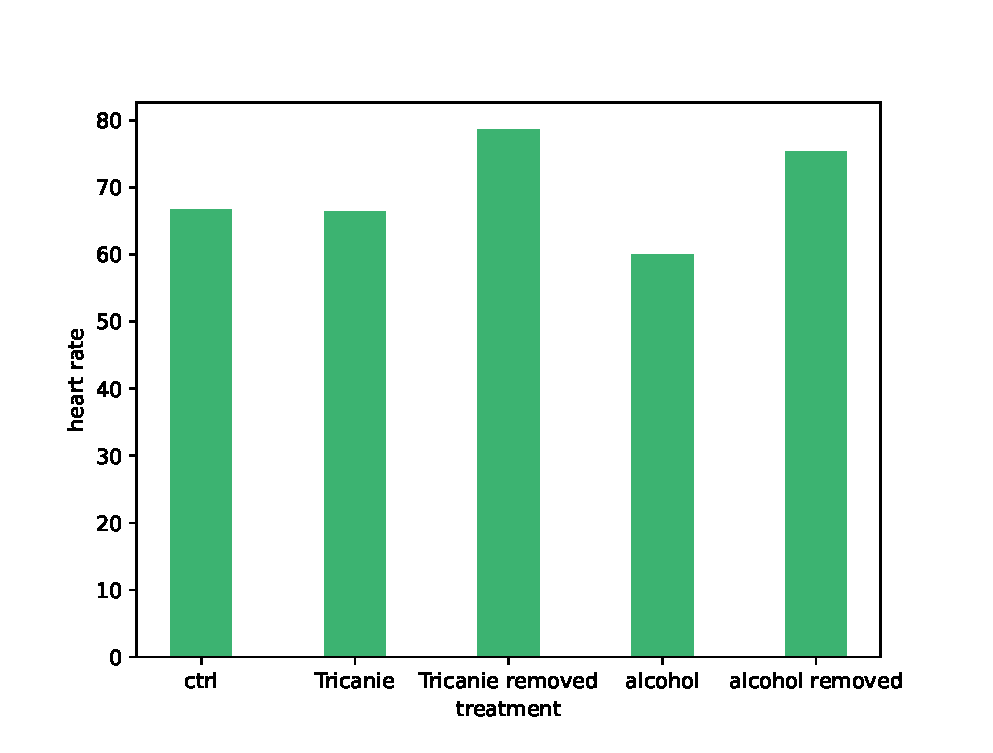
\includegraphics[scale = 0.5]{src/zoology/Figure1.eps}}
        \subfigure[]{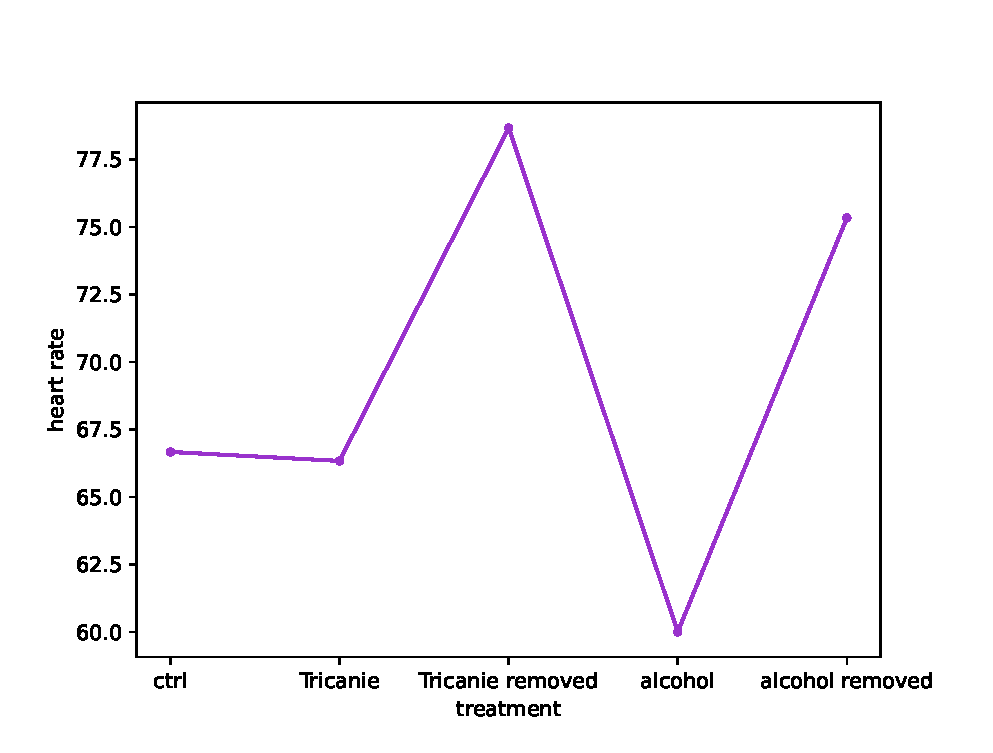
\includegraphics[scale = 0.5]{src/zoology/Figure2.eps}}
    \end{figure}
\end{document}